\documentclass{article}
\usepackage[utf8]{inputenc}
\usepackage[margin=1in]{geometry}
\usepackage{amsmath}
\setlength{\parindent}{0em}
\setlength{\parskip}{0.5em}
\usepackage{graphicx}
\usepackage{tabto}
\usepackage[table]{xcolor}
\usepackage{subcaption}
\usepackage{float}
\usepackage{wrapfig}

\title{CTA200 2020 Assignment 2}
\author{Yansong Qian}
\date{\today}

\begin{document}

\maketitle

\section*{Question 1}

\begin{figure}[H]
    
    \begin{subfigure}{7cm}
    \centering
    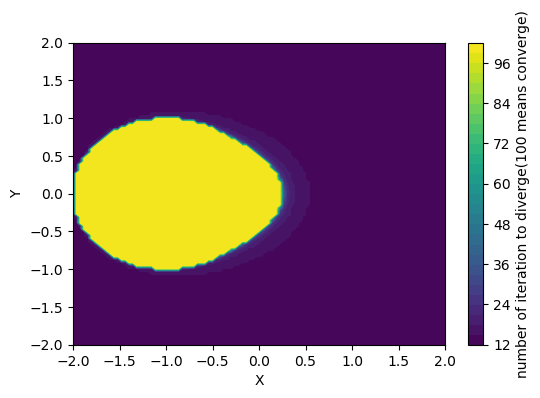
\includegraphics[width=7cm]{1.1.png}
    \caption{$-2 < x < 2$ and $-2 < y < 2$}
    \label{fig:my_label}
     \end{subfigure}
     \begin{subfigure}{7cm}
    \centering
    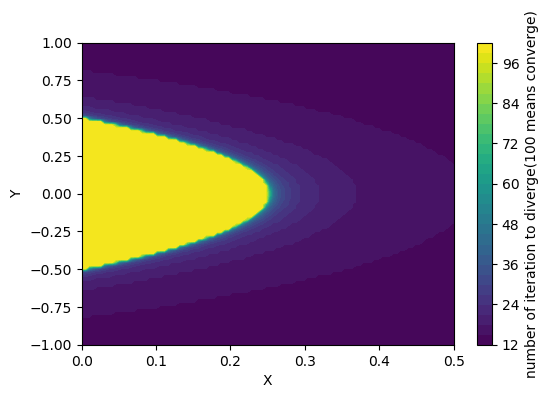
\includegraphics[width=7cm]{1.2.png}
    \caption{$0 < x < 0.5$ and $-1 < y < 1$}
    \label{fig:my_label}
     \end{subfigure}
     \caption{Divergence graph}
\end{figure}

\indent To produce the sequence $z_n$, I write a recursive python function. The function has two parameters n and c, where c is a complex number described in question. There are two possible types of output. If $z_n$ is finite, the function will return the complex number $z_n$. If $z_n$ is infinite, the function will return a list with only one element i, where i is the smallest integer between 0 and n where $z_i$ is infinite. To plot my result, I create a 2d array. One dimension is for real part and another dimension is for imaginary part. And I use my recursive function to calculate the iteration number where it converges for each point.\\
\\
\indent Figure 1(a) shows that the sequence will diverge if real part and imaginary part is large, but it is not likely to diverge if the real part of c is negative. Figure 1(b) is a zooming in version if (a) in the boundary. We can see if the real part is larger than 0.25, the sequence will diverge very quickly(less than 50 iteration). But if real part is smaller than 0,25, the sequence will not diverge after 100 iteration. 


\section*{Question 2}


\begin{figure}[H]
    
    \begin{subfigure}{7cm}
    \centering
    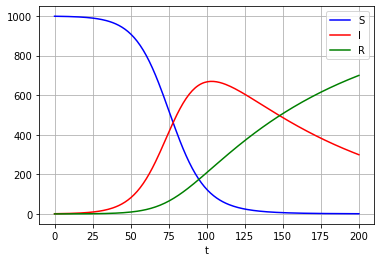
\includegraphics[width=7cm]{0.1&0.01.png}
    \caption{$\beta = 0.1, \gamma = 0.01$}
    \label{fig:my_label}
     \end{subfigure}
     \begin{subfigure}{7cm}
    \centering
    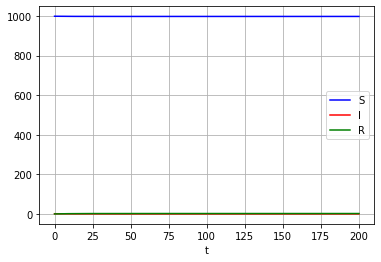
\includegraphics[width=7cm]{0.1&0.2.png}
    \caption{$\beta = 0.1, \gamma = 0.2$}
    \label{fig:my_label}
     \end{subfigure}
     \\
     \begin{subfigure}{7cm}
    \centering
    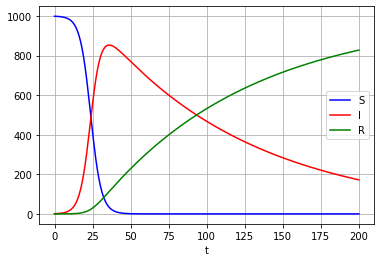
\includegraphics[width=7cm]{0.3&0.01.png}
    \caption{$\beta = 0.3, \gamma = 0.01$}
    \label{fig:my_label}
     \end{subfigure}
     \begin{subfigure}{7cm}
    \centering
    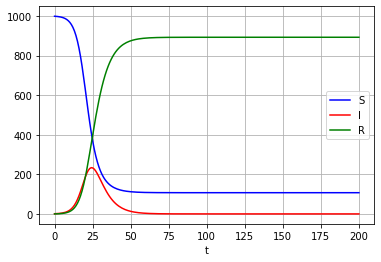
\includegraphics[width=7cm]{0.5&0.2.png}
    \caption{$\beta = 0.5, \gamma = 0.2$}
    \label{fig:my_label}
     \end{subfigure}
     \caption{SIR model solutions}
\end{figure}

\indent I use scipy.integrate.odeint to solve the ODE system. And use four different combination of $\beta$ and $\gamma$ to show different cases.\\
\\
\indent Overall, $\beta$ is the parameter related to infection rate and $\gamma$ is the parameter related to recovery rate. By comparing figure 2(a) and 2(c), we know higher infection rate will cause more rapid increase in infection number and also higher infection peak. Figure 2(b) shows that if recovery rate is higher than infection rate, the disease will not spread. 



\end{document}